%! program = pdflatex
%Carthage Physics Senior Thesis Template Rev. 2012
%Author:  Julie Dahlstrom

\documentclass[twocolumn,12pt]{article}
\usepackage[hmargin={1.25in,0.75in},bmargin=1in,tmargin=1in]{geometry} 
\usepackage{setspace}

% see geometry.pdf on how to lay out the page. There's lots.

% the following line enables graphics insertions (i.e. line art and photos). 
\usepackage{graphicx}

% the following line allows URLs to be handled gracefully
\usepackage{url}

% the following lines allow you to use some symbol fonts as necessary
\usepackage{mathtools}
\usepackage{gensymb}
\usepackage{amssymb}
\usepackage{float}

%  Use this next package to produce a more compact document if your LaTeX version includes it.  
%\usepackage[normalmargins,normalindent]{savetrees}

% %%%%%%%%%%%%%%%%%%%%%%%%%%
%
%  Here is where you start making changes
%
%  Modify the next lines accordingly  
%
%%%%%%%%%%%%%%%%%%%%%%%%%%%%%%%%%%%%%%

\title{This is my title:  \\
Fluid Mechanics}
\author{Aaron Scheets
%  Uncomment the next four lines when you are turning this in as a completed thesis
%\vspace{20pt}\\{\small\textit {A senior thesis submitted to the Carthage College Physics $\&$ Astronomy Department}}
%\vspace{0pt}\\{\small\textit {in partial fulfillment of the requirements for the Bachelor of Arts Degree in Physics}}
%\vspace{20pt}\\{Carthage College}
%\smallskip\\{Kenosha, Wisconsin}
}

%  Leave this line alone
\onecolumn

%%% End of header and beginning of document

\begin{document}

\maketitle

%The lines below enable some simple macros for equation display. 
\def\bd{\begin{displaymath}}
\def\be{\begin{equation}}
\def\ed{\end{displaymath}}
\def\ee{\end{equation}}

%  Leave the thesis double-spaced so your advisor can write nice expansive comments to help you in revisions.
\doublespacing

\begin{abstract} 
\noindent The abstract is a brief summary of all major sections of your thesis document.   It should appear on the cover page with the title and be followed by a page break.  Content of abstract should include a statement of what was done, the results that you obtained, and their significance.   The length of a good abstract should not exceed 150 words, typically.
\end{abstract}

\clearpage

% uncomment the line below to format the remainder of the document for  journal printing.
%\twocolumn 

\section{Introduction}

The goal of my thesis is to translate theory on fluid flow to computational models. To analytically model fluid flow, one must be able to relate the fluid properties, pressure, density, and temperature, and conserve mass, fluid momentum, and fluid energy. There exists a myriad of different flow types, and my thesis will concentrate on laminar, incompressible flow in particular. Laminar flow is non-turbulent and is therefore easier to solve for. To say that a flow is incompressible is to make the assumption that the fluid is of uniform density. Despite the existence of adequate fluid solvers, the abstraction of the details of the modeling process increases the probability of making poor assumptions when modeling a particular fluid flow.  

The introduction section should provide a broader context for your thesis topic that gradually narrows down to a thesis statement.  Think of the structure as a funnel:  start broad and end narrowly focused.  In your presentation, typically you will need to review prior work in the field in setting the stage for your current investigation.  Make sure you cite prior work appropriately.\cite{a-ref}

\subsection{Interesting Subtopic}

Use subsections to break sections down if you wish.  This technique can be very helpful if sections become long, especially in more substantial documents. Fig.\ref{dilate} illustrates how to insert and label figures.  (Note that LaTeX will keep track of numbering if you do it this way.) 

\begin{figure}
\begin{center}
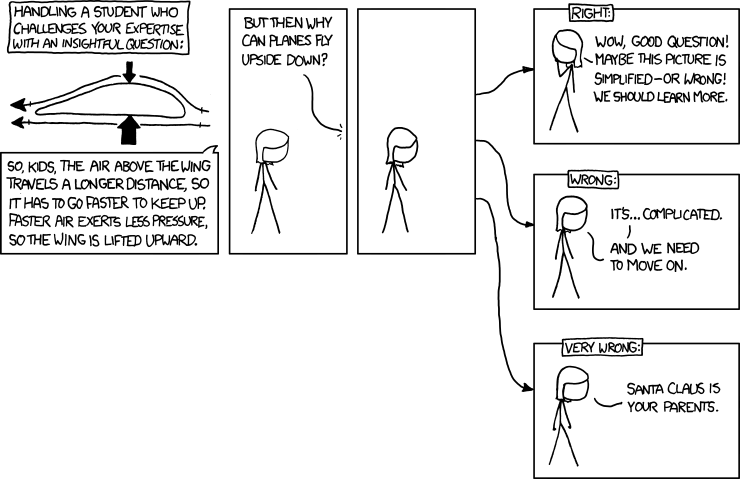
\includegraphics[width=6cm]{airfoil.png}
\caption{This is the caption for my figure, huzzah. \cite{c-ref}}
\label{fig:xkcdAirfoil}
\end{center}
\end{figure}

\subsection{Second Interesting Subtopic}

Subsections are like potato chips:  you can't have just one!  Maybe you will need to include a formula.  Here is an example of some gratuitous physics with a numbered equation on separate line as well as embedded in text.

A tree-level amplitude in $e^+e^-$ collisions can be expressed in
terms of fermion strings of the form
\begin{equation}
\bar v(p_2,\sigma_2)P_{-\tau}\hat a_1\hat a_2\cdots
\hat a_nu(p_1,\sigma_1) ,
\end{equation}
where $p$ and $\sigma$ label the initial $e^{\pm}$ four-momenta
and helicities $(\sigma = \pm 1)$, $\hat a_i=a^\mu_i\gamma_\nu$
and $P_\tau=\frac{1}{2}(1+\tau\gamma_5)$ is a chirality projection
operator $(\tau = \pm1)$.  The $a^\mu_i$ may be formed from particle
four-momenta, gauge-boson polarization vectors or fermion strings with
an uncontracted Lorentz index associated with final-state fermions.

For no particular reason, here is one last equation:
$ E = mc^2$.

%  Choose whichever one is appropriate
\section{Procedures}
%  \section{Experimental Design}  
This section details the actual investigation that you undertook in trying to answer your thesis question.  Your description may include description of an experimental set-up or it may involve showing steps of a detailed calculation.  Be thorough and specific in documenting what you did but avoid including the trivial (e.g. don't show numbers being plugged into equations).  Your goal should be documenting what you did in enough detail that someone else could duplicate the work without having to ``reinvent the wheel''. 

\section{Results}
You need to show your results in writing and also in a visual presentation (if appropriate).  Visuals may include tables of data, graphs, or images.  Be sure to document all columns of the tables and to provide figure captions.  Fig. \ref{ion} is a graph.

%% \begin{figure}[H]
%% \begin{center}
%% 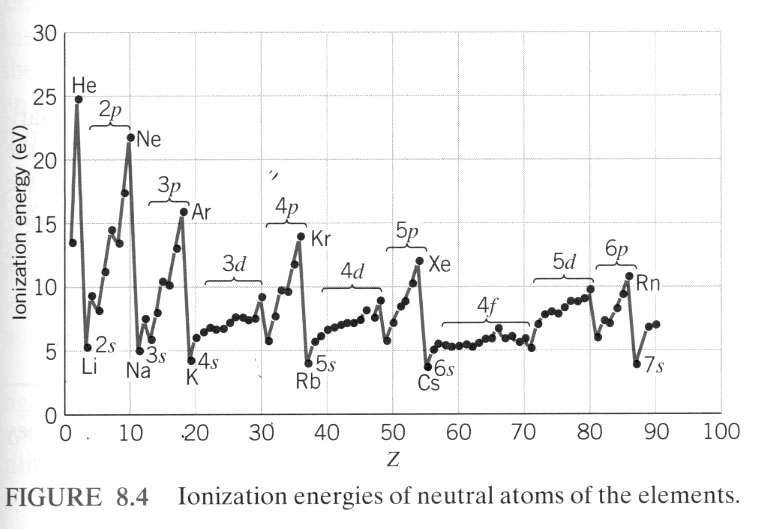
\includegraphics[width=13cm]{ionize_2d.jpg}
%% \caption{A plot of ionization energies for all elements in the periodic table.}
%% \label{ion}
%% \end{center}
%% \end{figure}


\section{Discussion}
Discuss the significance of your results within the larger context that you developed in the introduction section.  Note:  don't bother to try writing the discussion section before you have completed the study itself!  This is not only bad form, it's just plain a waste of time.


\section{Conclusion}
Don't forget to close your document with a conclusions section.  This is your opportunity to connect your far-reaching discussion section back to the task at hand:  answering the question you set for yourself.

\bibliography{libary.bib}
\bibliographystyle{ieeetr}


\begin{thebibliography}{99}

\bibitem{a-ref}Holman, T. (2008). Surround sound, up and running. Focal Press.
\bibitem{c-ref}Retrieved from \url{http://www.upscale.utoronto.ca/GeneralInterest/Harrison/GenRel/Images/TimeDilation5.gif}  
\end{thebibliography}

\section{Appendix}

Usually not needed, but just in case...

\section{Acknowledgements}
It's a nice gesture to thank people who have helped you in the thesis process.  If you received grant money to support your work or if you used certain on-line archives or databases, this is the place to put the standard boiler plate acknowledgement language.

\end{document}
